\documentclass{sigchi-ext}
% Please be sure that you have the dependencies (i.e., additional
% LaTeX packages) to compile this example.
\usepackage[T1]{fontenc}
\usepackage{textcomp}
\usepackage[scaled=.92]{helvet} % for proper fonts
\usepackage{graphicx} % for EPS use the graphics package instead
\usepackage{balance}  % for useful for balancing the last columns
\usepackage{booktabs} % for pretty table rules
\usepackage{ccicons}  % for Creative Commons citation icons
\usepackage{ragged2e} % for tighter hyphenation

% Some optional stuff you might like/need.
% \usepackage{marginnote}
% \usepackage[shortlabels]{enumitem}
% \usepackage{paralist}
% \usepackage[utf8]{inputenc} % for a UTF8 editor only

%% EXAMPLE BEGIN -- HOW TO OVERRIDE THE DEFAULT COPYRIGHT STRIP --
% \copyrightinfo{Permission to make digital or hard copies of all or
% part of this work for personal or classroom use is granted without
% fee provided that copies are not made or distributed for profit or
% commercial advantage and that copies bear this notice and the full
% citation on the first page. Copyrights for components of this work
% owned by others than ACM must be honored. Abstracting with credit is
% permitted. To copy otherwise, or republish, to post on servers or to
% redistribute to lists, requires prior specific permission and/or a
% fee. Request permissions from permissions@acm.org.\\
% {\emph{CHI'14}}, April 26--May 1, 2014, Toronto, Canada. \\
% Copyright \copyright~2014 ACM ISBN/14/04...\$15.00. \\
% DOI string from ACM form confirmation}
%% EXAMPLE END

% Paper metadata (use plain text, for PDF inclusion and later
% re-using, if desired).  Use \emtpyauthor when submitting for review
% so you remain anonymous.
\def\plaintitle{Breaking into new Data-Spaces: Infrastructure for Open Community Science}
\def\plainauthor{Aaron Halfaker, Jonathan Morgan, Yuvaraj Pandian, Elizabeth Thiry}
\def\emptyauthor{William Rand, Kristen Schuster, A.J. Million, Sean Goggins, David Laniado}
\def\plainkeywords{Open Collaboration Data Factories; Infrastructure; Methods; Policy; Online communities; Scientific practice}
\def\plaingeneralterms{Documentation, Standardization}

\title{Breaking into new Data-Spaces: Infrastructure for Open Community Science}

\numberofauthors{9}
% Notice how author names are alternately typesetted to appear ordered
% in 2-column format; i.e., the first 4 autors on the first column and
% the other 4 auhors on the second column. Actually, it's up to you to
% strictly adhere to this author notation.
\author{%
  \alignauthor{%
    \textbf{Aaron Halfaker}\\
    \email{ahalfaker@wikimedia.org} \\
    \textbf{Jonathan Morgan}\\
    \email{jmorgan@wikimedia.org} \\
    \textbf{Yuvaraj Pandian}\\
    \email{ypandian@wikimedia.org} \\
    \affaddr{Wikimedia Research} }\alignauthor{%
    \textbf{Kristen Schuster}\\
    \email{schuster.kristen@gmail.com} \\
    \textbf{A.J. Million}\\
    \email{ajmillion@gmail.com} \\
    \textbf{Sean Goggins}\\
    \email{GogginsS@missouri.edu} \\
    \affaddr{University of Missouri} } \vfil \alignauthor{%
    \textbf{Elizabeth Thiry}\\
    \affaddr{Boundless}\\
    \email{thirystheory@gmail.com } }\alignauthor{%
    \textbf{David Laniado}\\
    \affaddr{Digital Humanity}\\
    \affaddr{Eurecat}\\
    \email{david.laniado@gmail.com } } \vfil \alignauthor{%
    \textbf{William Rand}\\
    \affaddr{Robert H. Smith School of Business}\\
    \affaddr{University of Maryland}\\
    \email{wrand@umd.edu} }
}

% Make sure hyperref comes last of your loaded packages, to give it a
% fighting chance of not being over-written, since its job is to
% redefine many LaTeX commands.
\definecolor{linkColor}{RGB}{6,125,233}
\hypersetup{%
  pdftitle={\plaintitle},
%  pdfauthor={\plainauthor},
  pdfauthor={\emptyauthor},
  pdfkeywords={\plainkeywords},
  bookmarksnumbered,
  pdfstartview={FitH},
  colorlinks,
  citecolor=black,
  filecolor=black,
  linkcolor=black,
  urlcolor=linkColor,
  breaklinks=true,
}

% \reversemarginpar%

\begin{document}

\maketitle

% Uncomment to disable hyphenation (not recommended)
% https://twitter.com/anjirokhan/status/546046683331973120
\RaggedRight{}

% Do not change the page size or page settings.
\begin{abstract}
We propose a full day workshop focused on
experimentation with documentation protocols and
technologies that are designed to make the process
of ``breaking into'' a new dataset more tractible for 
researchers studying open online communities.
This workshop's purpose is to bring together researchers
to test these systems and discover problems and missed
opportunities to support iteration.  Participants
will also be given the opportunity to use state-of-the-art
documentation and technologies to break into a new collection
of datasets.  This workshop is the direct result of a call
to action to build infrastructure for data sharing
between researchers from past CSCW workshops and related
conferences.

\end{abstract}

\keywords{\plainkeywords}

\category{H.3.5}{Online Information Services}{Data sharing}
\category{H.3.4}{Systems and Software}{Information networks}

\section{Introduction}
Despite being easily accessible, open online community (OOC) data can be difficult to use effectively.  In order to access and analyze large amounts of data, researchers must first become familiar with the meaning of data values.  Then they must find a way to obtain and process the datasets to extract their desired vectors of behavior and content.  This process is fraught with problems that are solved (through great difficulty) over and over again by each research team/lab that \emph{breaks into} datasets for a new OOC.  Rarely does the description of methods presented in research papers provide sufficient depth of discussion to enable straightforward replication or extension studies.  Further, those without the technical skills to process large amounts of data effectively will often be prevented from even starting work.  The result of these factors is a set of missed opportunities around the promise of open data to expedite scientific progress.

In this workshop, we will experiment with strategies -- both technological systems and documentation strategies -- designed to enable our community to more thoroughly reap the benefits of open online data science practice.  We will invite participants to attempt the difficult work of breaking into a new dataset using tools and documentation designed to alleviate common difficulties.  In the months leading up to the workshop, we will prepare and describe several datasets within an open querying service and invite participants to explore these systems and their functionality through the replication and extension of a selected data-intensive research paper from past CSCW.  During the workshop participants will have the opportunity to explore new tools and datasets and to jump start new studies based on our curated documentation and infrastructure. As we observe and interact with our participants, we hope to learn from their successes and struggles and to use these learnings to iteratively improve our tools and documentation protocols.

This work builds on a call to action from a previous CSCW Workshops\cite{goggins14ocdata, morgan15advancing} and ongoing initiatives\footnote{\url{http://www.datafactories.org/}}: to build up shared research infrastructure\cite{wiggins14quality, morgan15advancing_report} to support data and method sharing practices. The workshop organizers come from many different backgrounds and have extensive experience with using OOC data, developing infrastructure to support access to and analysis of OOC data, and building communities of practice around OOC research.

We will use this workshop to achieve three goals:
\begin{enumerate}
\item identify common challenges and novel strategies for making open community research easier to replicate and extend -- specifically targeting protocols for documenting research methods (e.g. the ODD protocol\cite{grimm10odd})
\item inform the design of data management/analysis infrastructures like Quarry, our experimental open querying service\footnote{\url{https://meta.wikimedia.org/wiki/Research:Quarry}}
\item inform the design of metadata indexes like the Open Collaboration Data Factory's wiki\footnote{\url{http://wiki.urbanhogfarm.com/index.php/Main_Page}}
\end{enumerate}

We also hope to foster a community of practice within CSCW around open data management and plan for next steps towards accelerating scientific progress around the study of computer-supported cooperation just as past workshops have informed our plans for this workshop proposal.


\section{Using open online data}
Regretfully, the technical availability of OOC datasets has not been a panacea for the study of socio-technical phenomena in these communities.  Based on past research and workshops designed to help us explore OOC data science practices, we have identified three key hypotheses about what makes \emph{breaking into} new datasets so difficult: (1) methods descriptions are often insufficient as a guide to replication \& extension, (2) technological literacy bars access to processing large datasets, and (3) inconsistent and poorly indexed metadata prevent discovering what data is available and what the items of a dataset \emph{mean}.


\subsection{Methods replication}
OOC research has advanced considerably in the last few decades, but it is still difficult to compare and contrast research findings from different pieces of work.   Part of this is due to the very nature of the research; it comes from all sort of fields from information systems (e.g. \cite{ma07through}) to computer science (e.g. \cite{shneiderman00creating}) to information science (e.g. \cite{preece00online}) to marketing (e.g. \cite{kozinets02field}), and is studied in a wide variety of platforms from Twitter (e.g. \cite{vieweg10microblogging}) to Wikis (e.g. \cite{beschastnikh08wikipedian}) to question-and-answer forums (e.g. \cite{zhang07expertise}).  As a result, different disciplines and study venues use different language and descriptions, making it hard to integrate knowledge gleaned from disparate origins.

Moreover, the lack of easy translatability between fields and platforms has made the reproducing of findings difficult.  A researcher in one field use a definition used or understood the same way in another field.  For example, it's difficult for a researcher who works with Flickr data to understand how certain concepts are operationalized by researchers who work with blogging data. The field has progressed fine up until this point because there is so much research to do in this space, but now is the time to start building a cohesive theory of online communities and to create knowledge built on top of other knowledge, and to provide standards that allow different researchers to reproduce each others' findings.

In order to take the field to the next step, it is necessary to develop a standard of communication that will allow different researchers to communicate how and why they performed their analysis and research the way that they did.  One development in other interdisciplinary fields that has helped communication across boundaries is the creation of a uniform methods protocol (e.g. \cite{grimm10odd}).  By creating standards that describe how data is collected and analyzed, as well as how certain measurements in the theory are operationalized within the data, it is possible to make it easier for different researchers to understand each other's work and to reproduce findings.


\subsection{Technical literacy}
While there are many powerful, widely available, free/libre tools for gathering, manipulating, and analyzing large datasets, CSCW is an interdisciplinary field and  researchers' expertise for using these tools varies quite widely.  Even for researchers with such expertise, the beginning of a large-scale analysis is fraught with technical issues around formatting, types and structure and this results in a long process of trial and error. For researchers without such data engineering expertise these problems can seem intractable.  For example, at a past OOC data analysis workshop that we organized for the GROUP'15 conference, our expert participants spent 5 hours (the majority of the workshop day) converting and loading (100m row) datasets into an analysis framework that would allow the larger group to answer basic questions.  Even after the data was loaded, there were substantial concerns about inconsistencies between the documentations and the observed row counts.

With the goal of democratizing data analysis, we have been experimenting with open dataset interfaces that make the allow us to do such basic data engineering work up front and minimize the difficulty that future researchers experience when \emph{breaking into} the dataset.  We have identified two components that characterize open dataset interfaces: (1) public GUI sandboxes and query interfaces for lightweight in-situ data exploration and (2) approachable query languages (e.g. SQL).

We have developed such an open dataset interface for Wikimedia Datasets in the form of a public SQL querying service, called Quarry.  Quarry loads row-based datasets into a relational database management system and allows a user to join and filter datasets on the server through a web-based user interface.  This service allows both the direct download of datasets and download/sharing of secondary queries produced by queries.  We have found that non-experts can acquire proficiency in SQL over the course of an hour and that experts can use SQL powerfully.  Further, by making past queries public, newcomers are able to learn common and advanced querying strategies on their dataset of interest. This helps non-experts to quickly gain proficiency and, thus, become increasingly comfortable with new technologies that support their research agendas.

\begin{marginfigure}[-35pc]
  \begin{minipage}{\marginparwidth}
    \centering
    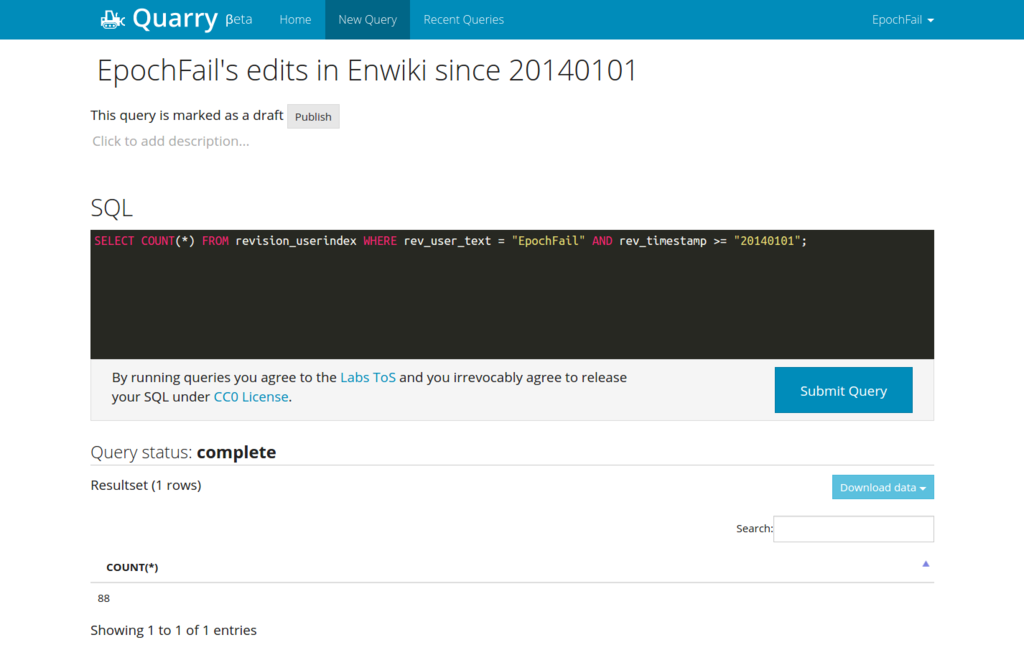
\includegraphics[width=0.9\marginparwidth]{figures/quarry}
    \caption{A screenshot of the Quarry public querying system}~\label{fig:marginfig}
  \end{minipage}
\end{marginfigure}

We see querying interfaces like these as a key opportunity to make OOC datasets more accessible to both data engineering experts and laypeople.  In this workshop, we'll put this conjecture to the test by supplying datasets through Quarry and learning from the experiences of participants.


\subsection{Metadata and taxonomies}
In order to \emph{break into} a new dataset, a researcher will need to discover it and determine know how to make use of it.  Currently, OOC datasets are scattered across various websites on the internet.  They are inconsistently (if at all) documented and the terms used to describe the characteristics of the data differ based on the discipline of the authors.  By gathering and standardizing information about OOC datasets, we can dramatically improve the discover-ability and utility of them.

Classifying OOC datasets so interdisciplinary researchers can discover, access, and use them in collaboration with other scholars requires consistent and agreed upon descriptions. Engaging these challenges in a CSCW workshop will allow us to articulate shared research goals, develop common terminology for describing datasets in generalizable terms, and determine how to document metadata at different descriptive levels so that OOC researchers can use these datasets effectively. 

OOC datasets can be described on three levels: the meta, mezzo and micro.  The meta-level is descriptive information that aids researchers in finding datasets and conducting a preliminary evaluation of their value prior to use.  This level also supports data management\footnote{\url{http://www.dcc.ac.uk/resources/curation-lifecycle-model}}.  The mezzo-level describes the meaning captured in a dataset's content.  Scholars use mezzo-level information to understand OOCs across disciplines, create theories, conduct scholarship, etc.  Last is micro-level dataset information, which granularly describes the contents and structure of a dataset. Tiered metadata schemas allow us to account for different research methods, modes of analysis, storage systems, and disciplinary norms and to support other considerations such as dataset accessibility (e.g. copyright) and research ethics.


\section{Workshop plan}
\input{sections/plan}

\subsection{Participation}
Participants will be recruited through a mixture of strategies.  We will contact participants from past workshops\cite{wiggins14quality, morgan15advancing, goggins14ocdata}.  We'll post announcements on social media (Twitter \& Facebook) as well as open science/HCI related listserves.  Participants will be selected based on their interest and experience working on OOC datasets.  We will be inclusive since we'd like to learn about opportunities to support a wide variety of research experience levels and expertise, but we will cap attendance at 50 participants because it would likely become difficult to manage after this point.

As we accept participants to the workshop we'll survey them to gather ideas for replication/extension studies that could be mostly completed in the context of a Workshop.  Participants will be asked to suggest a study to replicate/extend and describe what datasets and analysis would be necessary.


\subsection{Workshop preparation}
We'll gather and describe a small set of primary datasets relevant to the replication/extension study we plan to ask participants to run.  We'll supplement the methods descriptions of the paper we have chosen to replicate based on our proposed methods and metadata protocols.  As part of this work, we'll also perform our own replication in advance to know what time-intensive analyses are involved.  We'll take the opportunity to produce secondary datasets that would take too long to produce in the course of an 8 hour workshop day.

Datasets will be preloaded in our shared querying environment (Quarry) and metadata will be described in the OCDF metadata census wiki.  Both of these systems work as intended today, but we will continue to extend them and add features as the workshop approaches.


\subsection{Workshop day}
\textbf{Vision statement.} A short presentation and extended discussion about the purpose of the workshop and the larger initiative towards better infrastructure for open community data science.

\textbf{Hack session.} Participants (split into teams) work on the replication/extension task.  Participants will have a total of 4.5 hours' time on task besides introduction, breaks, and reflection time.  The workshop organizers will work with participants to both answer their questions and observe their work.

\textbf{Reporting and reflection.} Participant teams report on their progress and reflect on what did and did not work for them.  We will specifically ask how the methods description, querying system, and metadata was helpful and how.

\subsubsection{Schedule (tentative)}
\begin{itemize}
\item 8:15-9:00: breakfast mingling
\item 9:00 (sharp!): Intro to the day (process + brief task overview)
\item 9:10-10:00: Vision statement about Infrastructure for OOC studies
\item 10:00-10:15: Data introduction -- Each team/table reviews the task, documentation and infrastructure.
\item 10:15-10:30: coffee break, email breaktime
\item 10:30-12:00: Morning hack session breakouts (one team per table)
\item 12:00-12:30: Lunch serving, email breaktime
\item 12:30-3:15: Afternoon hack session breakouts (one team per table)
\item 3:15-3:30: coffee break, email breaktime
\item 3:30-4:30: Report-out and reflection
\item 4:30: Wrap-up, Thanks \& Next steps.
\item 5:00: Dinner discussion \& share contacts.
\end{itemize}


\subsection{Summary reporting}
At the end of the day, we will use the last hour as an opportunity for our participants to discuss what worked and what didn't.  We will capture their discussion points in a collaborative document that all participants will be invited to edit and extend.  We'll use these notes and our observations during the workshop to publish a report summarizing major take-aways to inform future work.


\balance{}

\bibliographystyle{SIGCHI-Reference-Format}
\bibliography{refs}

\end{document}

%%% Local Variables:
%%% mode: latex
%%% TeX-master: t
%%% End:
